\section*{Dati e risultati}

\subsection{Rilevatore di picchi}

In questa sezione ci occuperemo di verificare il corretto funzionamento di un circuito rilevatore di picchi costruito con un diodo 1N4007.
Il circuito che abbiamo utilizzato è schematizzato in Figura \ref{fig:circuito_peak}.
In questa configurazione abbiamo impostato che il valore di capacità ($C$) fosse di $1\,\si{\micro\farad}$, mentre il valore della resistenza $R_2$ fosse di $1\,\si{\kilo\ohm}$. Ricordiamo che sul valore della capacità abbiamo un incertezza nominale dell'$1\,\%$,mentre sulla resistenza vi è un errore nominale del $5\,\%$.
Il circuito è stato alimentato con una differenza di potenziale pico-pico in entrata di $10\,\si{\volt}$ ad una frequenza di $100\,\si{\hertz}$.

Quindi per verificare il corretto funzionamento del nostro rilevatore di picchi visuaizziamo la tensione in uscita ($V\ped{out}$) e ne studiamo l'andamento al variare di $C$ e della resistenza $R_1$.
Aggiungiamo che per semplificare le operazioni abbiamo deciso di variare la resistenza $R_1$ mantenedo costante la capacità, e di variare $C$ mantenendo costante $R_2$.
Di seguito riportiamo gli andamenti della tensione in uscita ($V\ped{out}$) al variare di $C$ e di $R_1$.

\begin{figure}[H]
    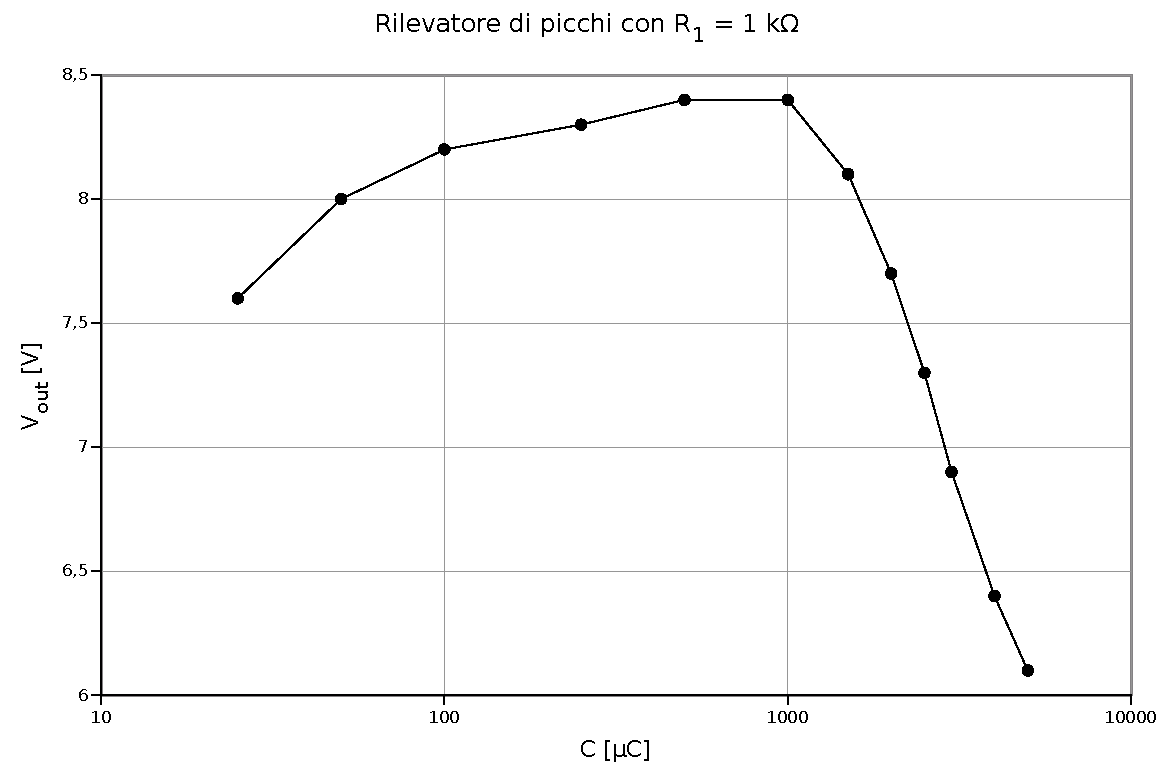
\includegraphics[scale=0.7]{capacita.pdf}
    \caption{}
    \label{fig:capacita}
\end{figure}

\begin{figure}[H]
    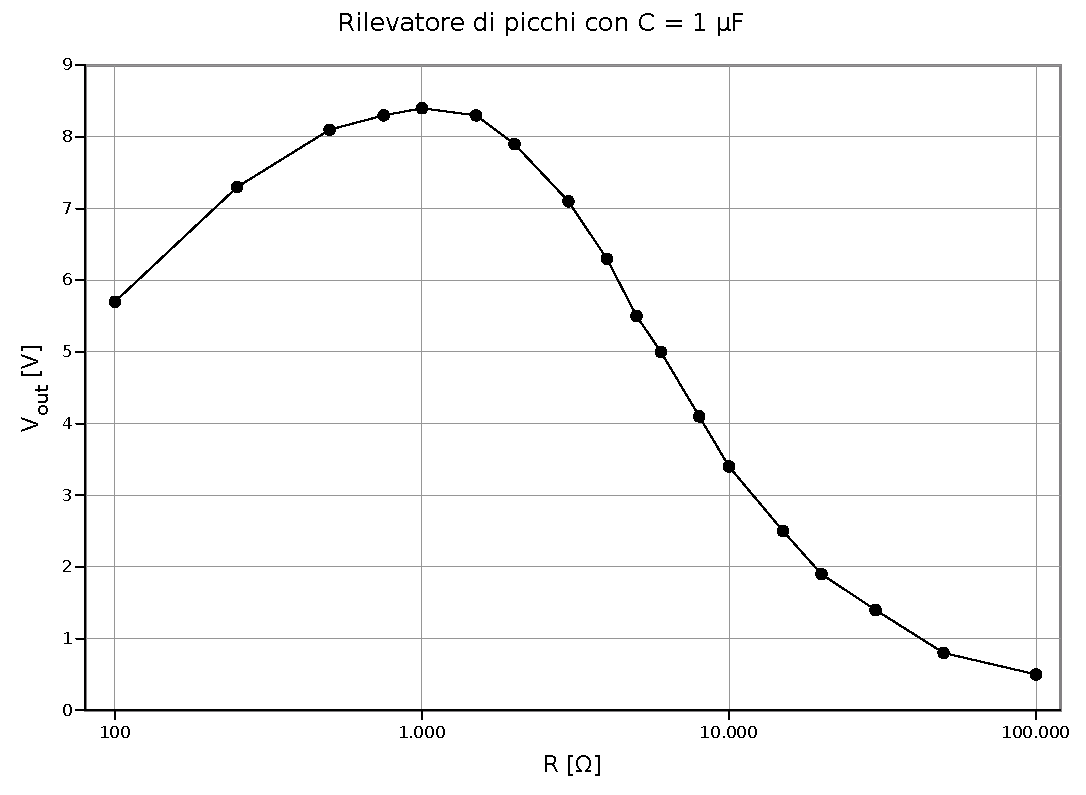
\includegraphics[scale=0.7]{resistenza.pdf}
    \caption{Andrea è un party dancer. Sono un fucking spammer.}
    \label{fig:resistenza}
\end{figure}

Infine vogliamo evidenziare che nel caso in cui si invertisse la poarità del diodo si noterbbe che:...

\subsection{Diodo Zener}

In questa seconda sezione vogliamo studiare la caratteristica $I-V$ in polarizzazione inversa del diodo Zener, modello XZY85C10 ed il suo uso come stabilizzatore di tensione.
Per studiarne la caratteristica $I-V$ abbiamo applicato ai capi del diodo Zener una tensione DC di $\pm\,25\,\si{\volt}$. 
Durante lo studio della caratteristca $I-V$ del diodo abbiamo tenuto conto della potenza massima dissipabile dal diodo. Infatti abbiamo fatto attenzione che il prodotto tensione-corrente non superasse mai la potenza ($W$) di $1\,\si{\watt}$, che è il valore massimo sopportabile dal nostro diodo.
I valori ottenuti sono riportati nel seguente grafico:

\begin{figure}[H]
    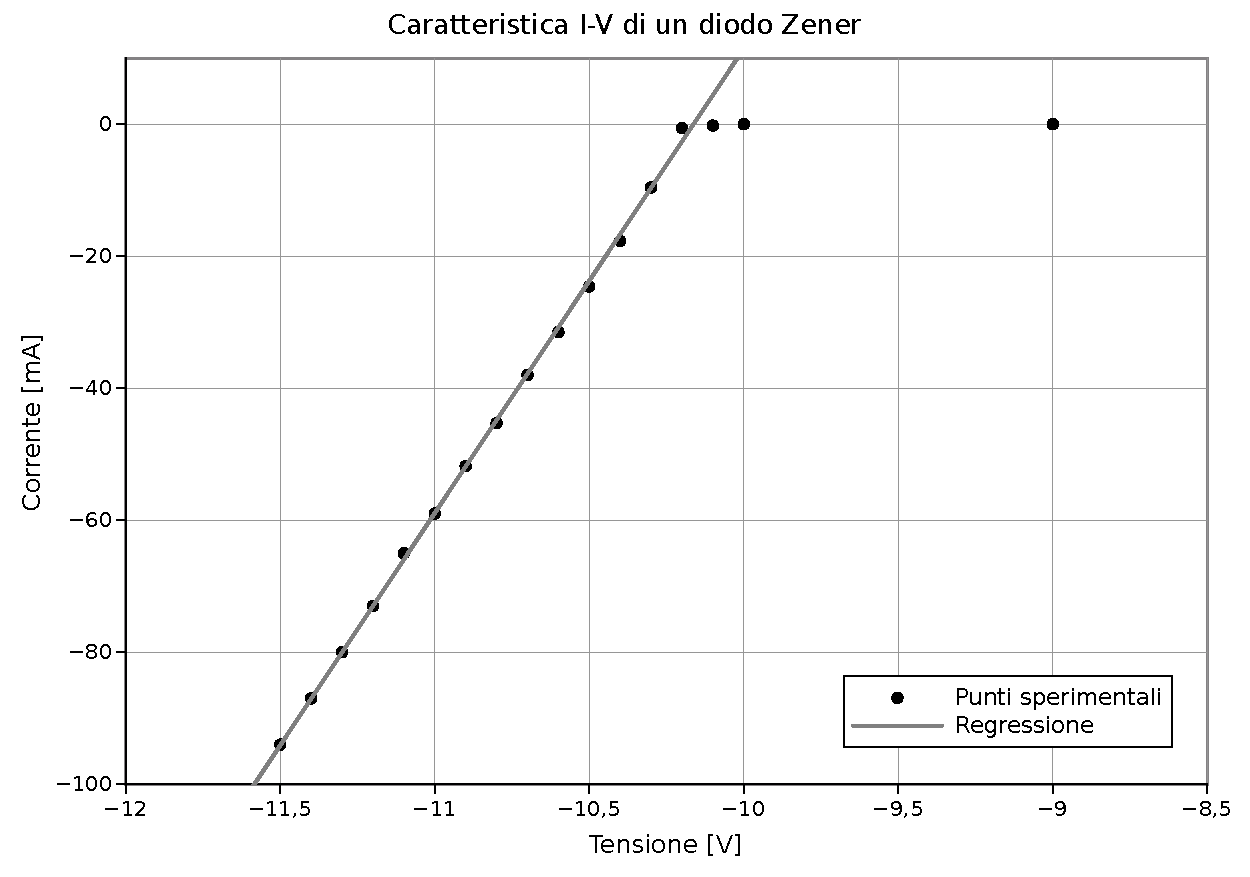
\includegraphics[scale=0.7]{cara_zener.pdf}
    \caption{Andrea è un party dancer. Sono un fucking spammer.}
    \label{fig:caratteristica_I-V}
\end{figure}

Inoltre abbiamo calcolato la resistenza dinamica ($R_d$) del diodo sfruttando la seguente relazione:

\begin{equation}
	R_d \,=\, \frac{\Delta V}{\Delta I} \,=\, 14.2\,\pm\,0.1 \,\,\si{\ohm}
\end{equation}

%14.209713510314533
%0.106189350778691

dove $\Delta V$ indica una differenza di potenziale e $\Delta I$ indica la differenza di intensità di corrente corrispondente. Inoltre facendo riferimento alla figura sopra riportata (Figura \ref{fig:caratteristica_I-V}) possiamo notare che la resistenza dinamica $R_d$ non è altro che l'inverso del coefficiente angolare della retta $I-V$ plottata.\\

Ottenute queste informazioni su questo modello di diodo Zener ci siamo proposti di determinare sperimentalmente, studiandone la caratteristica $I-V$, il range di funzionamento di tale componente elettronico se usato come stabilizzatore di tensione.
A tal fine abbiamo sfruttato il circuito illustrato in Figura \ref{fig:circuito_zener} che è stato alimentato con il generatore di tensione DC $\pm\,25\,\si{\volt}$ e la resistenza ($R$) applicatavi è di $1\,\si{\kilo\ohm}$.
I risultati da noi ottenuti sono riportati nel grafico sottostante:

\begin{figure}[H]
    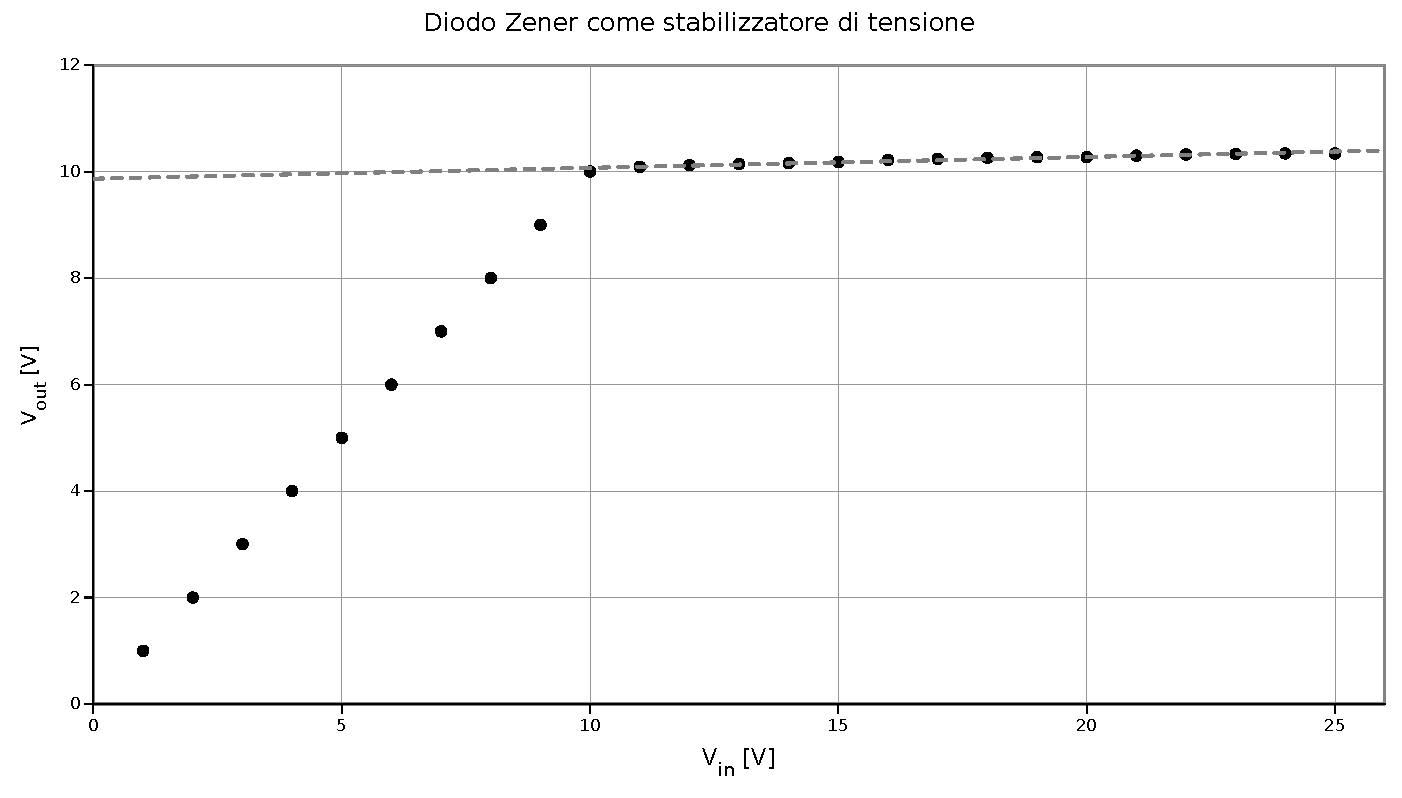
\includegraphics[scale=0.7]{stab.pdf}
    \caption{Andrea è un party dancer. Sono un fucking spammer.}
    \label{fig:stab_tensione}
\end{figure}

Infine vogliamo calcolare il raporto di stabilizzazione ($\chi$) sia teorico che sperimentale e verificarne la compatibilità.

\begin{equation}
	\chi\ped{exp} \,=\, \frac{\Delta V\ped{out}}{\Delta V\ped{in}} \,=\, 0.020\,\pm\,0.001
	\label{eq:c_exp}
\end{equation}

\begin{equation}
	\chi\ped{teo} \,=\, \frac{R_d}{R\,+\,R_d} \,=\, 0.0140\,\pm\,0.0006
	\label{eq:c_teo}
\end{equation}
